%!TEX root = main.tex
\vspace{-.0cm}
\section{Preliminaries}\label{sec:background}
\vspace{-1.22pt}
We recall some important concepts from Riemannian geometry. \citet{do2016differential}  provides more a thorough review, with \citet{absil2009optimization} providing a perspective particularly relevant for Riemannian optimization.

As a base space we consider a Riemannian manifold $(\M, \g)$--a smooth manifold equipped with a Riemannian metric $\g$ containing a compact, connected subset $\X$. At all $x \in \M$, the metric $\g$ induces a natural inner product on the tangent space $T_{x} \M$, denoted by $\langle\cdot,\cdot\rangle$--this inner product induces a norm on each tangent space denoted by $\Vert \cdot \Vert$. The metric $\g$ also provides a means of measuring the length of a parametrized curve from $\mathbb{R}$ to the manifold; a \emph{geodesic} is a constant speed curve $\gamma\! :\! [0,1]\! \to\! \M$ that is locally distance-minimizing with respect to the distance~$d$ induced by $\g$.

When considering functions $f : \M \to \mathbb{R}$ we will use $\nabla f(x) \in T_{x} M$ to denote the \emph{Riemannian gradient} of $f$ at $x \in \M$, and $\Hess f(x) : T_{x} M \to T_{x} M$, the \emph{Riemannian Hessian} of $f$ at $x$. When considering functions between manifolds $F : \M \to \M$, we will use $D F(x) : T_{x} \M \to T_{F(x)} \M$ to denote the \emph{differential} of the mapping at $x$ (its linearization) % for which the chain rule and inverse function theorem also hold
\citep[see][for more formal definitions of these objects]{absil2009optimization}.
 \begin{figure}[!t]
 \vspace{-.5cm}
\centering
\begin{minipage}[c]{.48\linewidth}
 \def\svgwidth{2.5in}
%!TEX root = ../colt2018-manifold.tex

%% Creator: Inkscape inkscape 0.92.2, www.inkscape.org
%% PDF/EPS/PS + LaTeX output extension by Johan Engelen, 2010
%% Accompanies image file 'retraction.pdf' (pdf, eps, ps)
%%
%% To include the image in your LaTeX document, write
%%   \input{<filename>.pdf_tex}
%%  instead of
%%   \includegraphics{<filename>.pdf}
%% To scale the image, write
%%   \def\svgwidth{<desired width>}
%%   \input{<filename>.pdf_tex}
%%  instead of
%%   \includegraphics[width=<desired width>]{<filename>.pdf}
%%
%% Images with a different path to the parent latex file can
%% be accessed with the `import' package (which may need to be
%% installed) using
%%   \usepackage{import}
%% in the preamble, and then including the image with
%%   \import{<path to file>}{<filename>.pdf_tex}
%% Alternatively, one can specify
%%   \graphicspath{{<path to file>/}}
%% 
%% For more information, please see info/svg-inkscape on CTAN:
%%   http://tug.ctan.org/tex-archive/info/svg-inkscape
%%
\begingroup%
  \makeatletter%
  \providecommand\color[2][]{%
    \errmessage{(Inkscape) Color is used for the text in Inkscape, but the package 'color.sty' is not loaded}%
    \renewcommand\color[2][]{}%
  }%
  \providecommand\transparent[1]{%
    \errmessage{(Inkscape) Transparency is used (non-zero) for the text in Inkscape, but the package 'transparent.sty' is not loaded}%
    \renewcommand\transparent[1]{}%
  }%
  \providecommand\rotatebox[2]{#2}%
  \ifx\svgwidth\undefined%
    \setlength{\unitlength}{198.42519685bp}%
    \ifx\svgscale\undefined%
      \relax%
    \else%
      \setlength{\unitlength}{\unitlength * \real{\svgscale}}%
    \fi%
  \else%
    \setlength{\unitlength}{\svgwidth}%
  \fi%
  \global\let\svgwidth\undefined%
  \global\let\svgscale\undefined%
  \makeatother%
  \begin{picture}(1,1)%
    \put(0,0){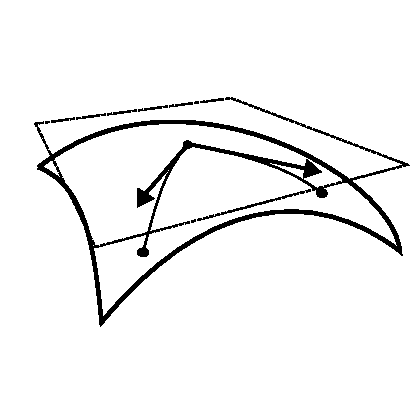
\includegraphics[width=\unitlength,page=1]{Figs/retractionbis.pdf}}%
    \put(0.47046491073,0.658059720226){\color[rgb]{0,0,0}\makebox(0,0)[lb]{\smash{$x_{n-1}$}}}%
     \put(0.75,0.60){\color[rgb]{0,0,0}\makebox(0,0)[lb]{\smash{$-\!\gamma_{n}\nabla f_{n}(x_{n-1})$}}}%
    \put(0.050473214,0.74160431){\color[rgb]{0,0,0}\makebox(0,0)[lb]{\smash{$T_{x_{n-1}}\M$}}}%
    \put(0.88081831845,0.328726181){\color[rgb]{0,0,0}\makebox(0,0)[lb]{\smash{$\M$}}}%
    \put(0.2809223052,0.47167483){\color[rgb]{0,0,0}\makebox(0,0)[lb]{\smash{$v$}}}%
     \put(0.780809223052,0.490167483){\color[rgb]{0,0,0}\makebox(0,0)[lb]{\smash{$x_{n}$}}}%
    \put(0.2207857,0.3651749994){\color[rgb]{0,0,0}\makebox(0,0)[lb]{\smash{$R_{x_{n\!-\!1}}\!(v)$}}}%
  \end{picture}%
\endgroup%

   \end{minipage}
   \begin{minipage}[c]{.48\linewidth}
 \def\svgwidth{2.5in}
%!TEX root = ../colt2018-manifold.tex

%% Creator: Inkscape inkscape 0.92.2, www.inkscape.org
%% PDF/EPS/PS + LaTeX output extension by Johan Engelen, 2010
%% Accompanies image file 'transport.pdf' (pdf, eps, ps)
%%
%% To include the image in your LaTeX document, write
%%   \input{<filename>.pdf_tex}
%%  instead of
%%   \includegraphics{<filename>.pdf}
%% To scale the image, write
%%   \def\svgwidth{<desired width>}
%%   \input{<filename>.pdf_tex}
%%  instead of
%%   \includegraphics[width=<desired width>]{<filename>.pdf}
%%
%% Images with a different path to the parent latex file can
%% be accessed with the `import' package (which may need to be
%% installed) using
%%   \usepackage{import}
%% in the preamble, and then including the image with
%%   \import{<path to file>}{<filename>.pdf_tex}
%% Alternatively, one can specify
%%   \graphicspath{{<path to file>/}}
%% 
%% For more information, please see info/svg-inkscape on CTAN:
%%   http://tug.ctan.org/tex-archive/info/svg-inkscape
%%
\begingroup%
  \makeatletter%
  \providecommand\color[2][]{%
    \errmessage{(Inkscape) Color is used for the text in Inkscape, but the package 'color.sty' is not loaded}%
    \renewcommand\color[2][]{}%
  }%
  \providecommand\transparent[1]{%
    \errmessage{(Inkscape) Transparency is used (non-zero) for the text in Inkscape, but the package 'transparent.sty' is not loaded}%
    \renewcommand\transparent[1]{}%
  }%
  \providecommand\rotatebox[2]{#2}%
  \ifx\svgwidth\undefined%
    \setlength{\unitlength}{198.42519685bp}%
    \ifx\svgscale\undefined%
      \relax%
    \else%
      \setlength{\unitlength}{\unitlength * \real{\svgscale}}%
    \fi%
  \else%
    \setlength{\unitlength}{\svgwidth}%
  \fi%
  \global\let\svgwidth\undefined%
  \global\let\svgscale\undefined%
  \makeatother%
  \begin{picture}(1,1)%
    \put(0,0){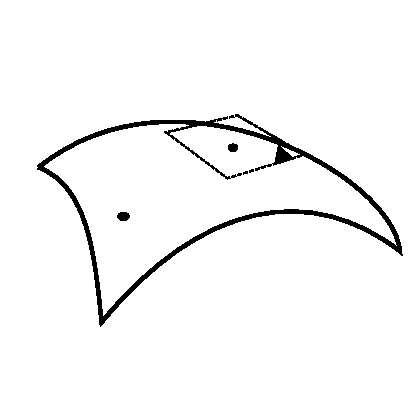
\includegraphics[width=\unitlength,page=1]{Figs/transport2.pdf}}%
    \put(0.88081831845,0.328726181){\color[rgb]{0,0,0}\makebox(0,0)[lb]{\smash{$\M$}}}%
    \put(0,0){\includegraphics[width=\unitlength,page=2]{Figs/transport2.pdf}}%
    \put(0.49373014,0.651988096){\color[rgb]{0,0,0}\makebox(0,0)[lb]{\smash{$x$}}}%
    \put(0.236627,0.47247038){\color[rgb]{0,0,0}\makebox(0,0)[lb]{\smash{$y$}}}%
    \put(0.1720032738,0.6014499){\color[rgb]{0,0,0}\makebox(0,0)[lb]{\smash{$T_y\M$}}}%
    \put(0.594176587,0.7369925609){\color[rgb]{0,0,0}\makebox(0,0)[lb]{\smash{$T_x\M$}}}%
    \put(0.70539679,0.56444469){\color[rgb]{0,0,0}\makebox(0,0)[lb]{\smash{$v$}}}%
    \put(0.42325397,0.4704097231){\color[rgb]{0,0,0}\makebox(0,0)[lb]{\smash{$\tp{x}{y}(v)$}}}%
  \end{picture}%
\endgroup%

  \end{minipage}
  \vspace{-1cm}
\caption{Left: In the tangent space at iterate $x_{n-1}$, a retraction along an arbitrary vector $v$ generating a curve pointing in the ``direction'' of  $v$, and a retraction along the gradient update to $x_n$. Right:
The parallel transport of a different $v$ along the same path.}
\label{fig:manifold}
  \vspace{-.5cm}
\end{figure}
The \emph{exponential map} $\Exp_{x}(v) : T_{x} \M \to \M$ maps $v \in T_{x} \M$ to $y \in \M$ such that there is a geodesic with $\gamma(0)=x$, $\gamma(1)=y$, and $\frac{d}{dt}\gamma(0)=v$; although it may not be defined on the whole tangent space. If there is a unique geodesic connecting $x, y \in \X$, the exponential map will have a well-defined inverse $\Exp_{x}^{-1}(y) : \M \to T_{x}\M$, such that the length of the connecting geodesic is $d(x,y)=\Vert \Exp_{x}^{-1}(y) \Vert$. We also use $R_x : T_{x} \M \to \M$ and $R_x^{-1} : \M \to T_{x}\M$ to denote a \emph{retraction mapping} and its inverse (when well defined), which is an approximation to the exponential map (and its inverse). $R_x$ is often computationally cheaper to compute then the entire exponential map $\Exp_x$. Formally, the map $R_x$ is defined as a first-order retraction if $R_x(0) = x$ and $D R_x(0)= id_{T_{x} \M}$---so locally $R_x(\xi)$ must move in the ``direction'' of $\xi$. The map $R_x$ is a second-order retraction if $R_x$ also satisfies $\frac{D^2}{dt^2} R_x(t \xi)|_{0} = 0$ for all $\xi \in T_{x}\M$, where $\frac{D^2}{dt^2}\gamma = \frac{D}{dt} \dot{\gamma}$ denotes the acceleration vector field \citep[][Sec.~5.4]{absil2009optimization}. This condition ensures $R_x$ satisfies a ``zero-acceleration'' initial condition.
Note that locally, for $x$ close to $y$, the retraction satisfies $\norm{R^{-1}_{x}(y)} = d(x, y) + o(d(x, y))$.

If we consider the example where the manifold is a sphere (i.e., $\M = S^{d-1}$ with the round metric $\g$), the exponential map along a vector will generate a curve that is a great circle on the underlying sphere. A nontrivial example of a retraction $R$ on the sphere can be defined by first moving along the tangent vector in the embedded Euclidean space $\mathbb{R}^d$, and then projecting this point to the closest point on the sphere.

We further define the \emph{parallel translation} $\tp{x}{y} : T_x \mathcal{M} \to T_y \mathcal{M}$ as the map
transporting a vector $v \in T_x \M$ to $\tp{x}{y} v$, along a path $R_{x}(\xi)$ connecting $x$ to $y = R_{x}(\xi)$, such that the vector stays ``constant" by satisfying a zero-acceleration condition. This is illustrated in \myfig{manifold}. The map $\tp{x}{y}$ is an isometry. We also consider, a different vector transport map $\te{x}{y}:T_x \mathcal{M} \to T_y \mathcal{M}$ which is the differential  $DR_{x}(R_x^{-1}(y))$ of the retraction $R$ \citep[][Sec.~8.1]{absil2009optimization}.

Following \citet{huang2015broyden}, we will call a function $f$ on $\X$ \emph{retraction convex} on $\X$ (with respect to $R$) if for all $x \in \X$ and all $\eta \in T_{x}\M$ satisfying $\norm{\eta}=1$, $t \mapsto f(R_{x}(t \eta))$ is convex for all $t$ such that $R_{x}(t \eta) \in \X$; similarly $f$ is \emph{retraction strongly convex} on $\X$ if $t \mapsto f(R_{x}(t \eta))$ is strongly convex under the same conditions. If $R_x$ is the exponential map, this reduces to the definition of geodesic convexity \citep[see the work of][for further details]{zhang2016first}.
\vspace{-1.21pt}
\section{Assumptions} \label{sec:assumptions}
\vspace{-1.22pt}
We introduce several assumptions on the manifold $\M$, function $f$, and the noise process $\{\nabla f_n\}_{n\geq1}$ that will be relevant throughout the paper.
\vspace*{-.1850cm}
\subsection{Assumptions on $\M$}
\vspace{-.0856cm}
First, we assume the iterates of the algorithm in \eq{grad_desc} and \eq{ave_grad_desc}
remain in $\mathcal X$ where the manifold ``behaves well.'' Formally,
\vspace*{-4pt}
\begin{assumption} \label{assump:manifold}
  For a sequence of iterates $\{ x_n \}_{n \geq 0}$ defined in \eq{grad_desc}, there exists a compact, connected subset $\mathcal X$ such that $x_n \in \mathcal X$ for all $n \geq 0$, and $x_\star \in \mathcal X$. Furthermore, $\mathcal X$ is totally retractive (with respect  to the retraction $R$) and the function $x\mapsto \Vert \frac{1}{2} R_y^{-1}(x)\Vert^2$ is retraction strongly convex on $\X$ for all $y\in\X$. Also, $R$ is a second-order retraction at $x_\star$.
\end{assumption}
\vspace*{-4pt}
Assumption~\ref{assump:manifold} is restrictive, but standard in prior work on stochastic approximation on manifolds \cite[e.g.,][]{bonnabel2013stochastic, zhang2016riemannian, sato2017riemannian}.
As further detailed by \citet{huang2015broyden}, a totally retractive neighborhood $\X$ is such that
for all $x \in \X$ there exists $r>0$ such that $\X \subset R_{x} (\mathbb{B}_{r}(0))$
where $R_x$ is a diffeomorphism on $\mathbb{B}_{r}(0)$. A totally retractive neighborhood is analogous to the concept of a totally normal neighborhood \citep[see, e.g.,][Chap. 3, Sec. 3]{do2016differential}.
Principally, Assumption~\ref{assump:manifold} ensures that the retraction map (and its respective inverse) are well-defined when applied to the iterates of our
algorithm.

If $\M$ is a Hadamard manifold, the exponential map (and its inverse) is defined everywhere on~$\M$, although this globally may not
be true for a retraction $R$. Similarly, if $\M$ is a compact manifold the first statement of Assumption~\ref{assump:manifold} is always satisfied. Moreover, in the case of the exponential map, $x \mapsto \frac{1}{2} \Vert \Exp_y^{-1}(x)\Vert^2$ is strongly convex in a ball around $y$
whose radius depends on the curvature, as explained by \citet{Afs11} and \citet[Ch. IV, Sec. 2 Lemma 2.9]{Sak96}. For our present purpose, we also assume the retraction $R$ agrees with the Riemannian exponential map up to second order near $x_\star$. This assumption, that $R$ is a second-order retraction, is fairly general and is satisfied by projection-like retraction maps on matrix manifolds \citep[see][]{AbsMal12}.
\vspace*{-.8cm}
\subsection{Assumptions on $f$}
\vspace{-.0856cm}
We now introduce some regularity assumptions on the function $f$ ensuring
sufficient differentiability and strong convexity at $x_\star$:
\begin{assumption} \label{assump:strongconvpoint}
The function $f$ is twice-continuously differentiable on $\X$. Further
the Hessian of the function $f$ at $x_\star$, $\Hess f(x_\star)$, satisfies,
for all $v \in T_{x_\star}\M$ and $\mu>0$,
\[
\langle v, \Hess f(x_\star)v\rangle \geq \mu \Vert v\Vert^2>0.
\]
\end{assumption}
Continuity of the Hessian  also ensures local retraction strong convexity in a neighborhood of $x_\star$ \citep[][Prop. 5.5.6]{absil2009optimization}. Moreover, since the function $f$ is twice-continuously differentiable on $\X$ its Hessian is Lipschitz on this compact set.
We formalize this as follows:
\begin{assumption}  \label{assump:HessianLip}
 There exists $M>0$ such that the Hessian of the function $f$, $\Hess f$, is $M$-Lipschitz  at $x_\star$.
That is, for all $y \in \X$ and $v \in T_{y}\M$,
\[
\Vert \tp{y}{x_\star}  \circ \Hess f(y) \circ \tp{x_\star}{y} -  \Hess f(x_\star)\Vert_{op} \leq M \Vert R_{x_\star}^{-1}(y) \Vert.
\]
\end{assumption}
Note that $\Vert R_{x_\star}^{-1}(y) \Vert$ is not necessarily symmetric under the exchange of $x_\star$ and $y$. This term could also be replaced with $d(x_\star, y)$, since these expressions will be locally equivalent
in a neighborhood of $x_\star$, but would come at the cost of a less transparent analysis.
\vspace{-0.11pt}
\subsection{Assumptions on the noise} \label{sec:assumptions_noise}
\vspace{-.0856cm}
We state several assumptions on the noise process that will be relevant throughout our discussion.
Let $(\F_n)_{n \geq 0}$ be an increasing sequence of sigma-fields. We will assume access to a sequence $\{\nabla f_n\}_{n \geq 1}$
of noisy estimates of the true gradient $\nabla f$ of the function $f$,
\begin{assumption} \label{assump:noiseunbiased}
The sequence of (random) vector fields $\{ \nabla f_n \}_{n\geq1} : \mathcal M \to T\mathcal M$ is $\F_n$-measurable, square-integrable and unbiased:
    \[
\forall x \in \X, \ \forall n \geq 1, \ \E[\nabla f_n(x)\vert \F_{n-1}]=\nabla f(x).
\]
\end{assumption}
This general framework subsumes two situations of interest.
\begin{itemize}
 \vspace*{-6pt}
 \item
Statistical Learning (on Manifolds): minimizing a loss function $\ell: \mathcal M \times  \mathcal Z \to \mathbb R$ over $x \in \mathcal X$, given a sequence
of i.i.d. observations in $\mathcal Z$, with access only to noisy, unbiased estimates of the gradient $\nabla f_n=\nabla \ell(\cdot,z_n)$ \citep{AswBicTom11}.
\vspace*{-6pt}
\item
Stochastic Approximation (on Manifolds): minimizing a function $f(x)$ over $x \in \mathcal X$, with access only to the
(random) vector field $\nabla f(x) + \epsilon_n(x)$ at each iteration. Here the gradient vector field is perturbed
 by a square-integrable martingale-difference sequence (for all $x\in\mathcal M $, $\E[\epsilon_n(x) \vert \F_{n-1}]=0$) \citep{bonnabel2013stochastic}.
\end{itemize}
Lastly, we will assume the vector fields $\{\nabla f_n\}_{n \geq 1}$ are individually Lipschitz and have
bounded covariance at the optimum $x_\star$:
\vspace*{-4pt}
\begin{assumption} \label{assump:noiseLip}
 There exists $L > 0$ such that for all $x \in \mathcal X$ and $n\geq 1$, the vector field $\nabla f_n$ satisfies
\[ \E [\Vert  \tp{x}{x_\star} \nabla f_n(x)- \nabla f_n(x_\star)\Vert^2\vert  \F_{n-1}]\leq L^2 \ \Vert R_{x_\star}^{-1}(x) \Vert^2 ,
 \]
there exists $\tau>0$ such that $ \E [\Vert  \nabla f_{n}(x) \Vert^4\vert  \F_{n-1}]\leq \tau^4$ for all $x \in \X$, and a symmetric positive-definite matrix $\Sigma$ such that,
 \[
 \E[\nabla f_n(x_\star) \otimes \nabla f_n(x_\star) \vert\mathcal F_{n-1}] = \Sigma \text{ a.s.} \]
\end{assumption}
These are natural generalizations of standard assumptions in the optimization literature \citep{Fab68} to the setting of
Riemannian manifolds\footnote{Assuming bounded gradients does not contradict Assumption~\ref{assump:strongconvpoint}, since we are constrained to the compact set $\X$.}. Note that the assumption, \\ $\E[\nabla f_n(x_\star) \otimes \nabla f_n(x_\star) \vert\mathcal F_{n-1}] = \Sigma \text{ a.s.}$ could be slightly relaxed (as detailed in \myapp{conv_rates}),
but allows us to state our main result more cleanly.
